\documentclass[sigconf]{acmart}

\setcopyright{acmlicensed}
\copyrightyear{2027}
\acmConference[ASP-DAC '27]{Asia and South Pacific Design Automation Conference}{January 2027}{}
\acmYear{2027}
\acmISBN{}
\acmDOI{}

\usepackage{tikz}
\usetikzlibrary{positioning,arrows.meta,fit,backgrounds,calc}
\usepackage{booktabs}
\usepackage{enumitem}

% Hard stop for text slipping past column margins: let LaTeX stretch
% interword spaces further before it resorts to an overfull (overflowing) line.
\usepackage{microtype}
\emergencystretch=3em
\sloppy

% Don't stretch inter-paragraph space to fill columns to equal height;
% avoids large gaps above section headings near column breaks.
\raggedbottom

% With raggedbottom, columns can end at different heights, which otherwise
% strands footnotes right under the shorter column instead of the page
% bottom. Pin footnotes to the true bottom of the page regardless.
\usepackage[bottom]{footmisc}

% palette, matching src/visualization/palette.py
\definecolor{pINK}{HTML}{3a352d}
\definecolor{pSUBINK}{HTML}{6f6757}
\definecolor{pCREAM}{HTML}{f4efe6}
\definecolor{pCHANNEL}{HTML}{ddd4c2}
\definecolor{pZERO}{HTML}{b8ad99}
\definecolor{pTERRA}{HTML}{c0603a}
\definecolor{pTEAL}{HTML}{3f6f74}
\definecolor{pSAGE}{HTML}{93a98d}
\definecolor{pSAND}{HTML}{cba14e}
\definecolor{pGRAY}{HTML}{a89f8d}
\definecolor{pRECLAIM}{HTML}{d8c19a}

% --- GA-on-softmax result, from the completed convergence run
% (ga_softmax_result.json: best_adpp/baseline_adp reduction 14.622%).
\newcommand{\GAred}{14.62}

\title{Amortized eFPGA Layout Search via Reinforcement Learning: Zero-Shot Generalization Across Circuit Topologies}

\author{First Author}
\email{firstname@university.edu}
\affiliation{%
  \institution{University Name}
  \city{City, State}
  \country{Country}
}

\author{Second Author}
\email{secondname@university.edu}
\affiliation{%
  \institution{University Name}
  \city{City, State}
  \country{Country}
}

\author{Third Author}
\email{thirdname@university.edu}
\affiliation{%
  \institution{University Name}
  \city{City, State}
  \country{Country}
}

\begin{document}

\begin{abstract}
Field-Programmable Gate Arrays (FPGAs) offer essential hardware flexibility
through programmable logic and interconnects. Embedded FPGAs (eFPGAs) extend
this capability by integrating reconfigurable fabrics directly into
fixed-silicon Systems-on-Chip (SoCs) or ASICs, enabling post-fabrication
functional updates and robust IP security. Hence, discovering optimized
layouts for these reconfigurable fabrics is essential to fully realize their
architectural potential. We train a single
graph-and-grid-conditioned Reinforcement Learning (RL) policy across various
benchmark circuits to place heterogeneous blocks (H-blocks, such as DSPs and
BRAMs) and select the optimal fabric aspect ratio for the eFPGA
architectures. We thereby generate layouts jointly optimized for Power,
Performance, and Area (PPA). To demonstrate generalizability, we evaluate
the trained RL policy on benchmark circuits completely unseen during
training, producing highly efficient zero-shot layouts. Across three random
seeds, the policy achieves up to a $58.73\%$ zero-shot ADP reduction on
unseen benchmark circuits relative to traditional island-style
architectures.
\end{abstract}

\keywords{FPGA, Reinforcement Learning (RL), Graph Convolutional Networks (GCN),
Convolutional Neural Networks (CNN), Macro Placement, Reconfigurable
Computing}

\begin{CCSXML}
<ccs2012>
   <concept>
       <concept_id>10010583.10010682.10010697</concept_id>
       <concept_desc>Hardware~Physical design (EDA)</concept_desc>
       <concept_significance>500</concept_significance>
       </concept>
   <concept>
       <concept_id>10010147.10010257.10010258.10010261</concept_id>
       <concept_desc>Computing methodologies~Reinforcement learning</concept_desc>
       <concept_significance>300</concept_significance>
       </concept>
   <concept>
       <concept_id>10010583.10010600.10010628</concept_id>
       <concept_desc>Hardware~Reconfigurable logic and FPGAs</concept_desc>
       <concept_significance>300</concept_significance>
       </concept>
 </ccs2012>
\end{CCSXML}

\ccsdesc[500]{Hardware~Physical design (EDA)}
\ccsdesc[300]{Computing methodologies~Reinforcement learning}
\ccsdesc[300]{Hardware~Reconfigurable logic and FPGAs}

\maketitle


\section{Introduction}
\label{sec:intro}

A generic FPGA inherently over-provisions hardware resources for any single
application, carrying extra routing and heterogeneous blocks
(\emph{H-blocks}: DSP slices, BRAMs) that the deployed netlist never fully
utilizes. Sizing an eFPGA fabric for one specific netlist recovers much of
this overhead. The product of routing area, critical-path delay, and total
power (\textbf{ADP} throughout) directly quantifies this overhead; minimizing
this metric benefits every eFPGA application~\cite{golds,nsgaii}.\footnote{GOLDS~\cite{golds}
uses the same abbreviation, ADP, for a different, two-term
(logical\_area$\times$delay) product; the proposed framework employs a
three-term (routing\_area$\times$delay$\times$power) product throughout this
paper.}

Prior efforts optimize fabric layouts on a per-design basis using
computationally expensive search heuristics like Genetic Algorithm (GA)~\cite{golds}
or NSGA-II~\cite{nsgaii}. These approaches restart the search from scratch
for every new circuit, transferring no knowledge across runs and incurring
the full computational search cost each time.

We train a single graph-and-grid-conditioned RL policy to
determine H-block placement and fabric aspect ratio, addressing a domain
where computationally expensive per-instance GA search previously served as
the only option. Unlike RL methods~\cite{rlplace,vprgym} that assign blocks to a pre-fabricated
grid, our policy directly constructs the fabric layout itself. After
jointly training on 11 circuits evaluated via the standard VTR flow, we
apply a single model checkpoint zero-shot to unseen circuits, including
fabrics up to $3.4\times$ the maximum training pool area. We train only
once, after which evaluating a new circuit requires just a single policy
rollout.
We compare against a from-scratch GA under an identical oracle, metric, and
baseline: the GA retains a higher absolute ADP reduction on some circuits,
but each of its generations requires its own VTR call, a cost that grows
with circuit size. The zero-shot policy requires a single VTR call per
circuit, so its relative advantage grows on the larger circuits where the
GA's search cost is highest (Section~\ref{sec:results-ga}).

\noindent We contribute:
\begin{itemize}[topsep=2pt,itemsep=2pt,leftmargin=2em]
  \item A graph-and-grid-conditioned RL policy that \emph{constructs} the
        eFPGA fabric itself, placing H-blocks and selecting fabric aspect
        ratio, rather than assigning blocks to an already-fabricated grid
        as prior RL placement methods do.
  \item An amortized alternative to per-instance GA/NSGA-II search:
        training cost is incurred once and reused through a single rollout
        per new circuit, whereas evolutionary search restarts from scratch
        for every design.
  \item A multi-modal feature extractor combining a GNN encoding of the
        netlist graph with a CNN encoding of the occupancy grid, giving the
        policy a fixed action space and the inductive bias for
        cross-topology transfer across varying netlist sizes and H-block
        counts.
\end{itemize}

\section{Background and Related Work}
\label{sec:related}

\subsection{Per-Design eFPGA Layout}

This over-provisioning (Section~\ref{sec:intro}) motivates fitting tile
placement and fabric dimensions to one specific netlist for a compact,
efficient fabric. Applications include IP security
(function absent from fixed silicon until configured~\cite{alice,arianna}),
domain-specific acceleration, and post-fabrication reconfigurability~\cite{golds}.
Subsequent work reduces overhead by shrinking under-utilized routing~\cite{shell}
or de-regularizing the fabric~\cite{nuredact}, both motivating the
non-island-style layouts we synthesize. All rely on per-design
search; none amortizes layout effort across netlists.
GOLDS~\cite{golds} introduced layout search built for a single design: a GA over
H-block placement with Area$\times$Delay fitness through the real VTR flow.
A follow-up~\cite{nsgaii} applies NSGA-II, also co-evolving CLB LUT size
and H-block sizing. Both report per-design gains on their own two-term
Area$\times$Delay metric, a different quantity from the three-term ADP
we report. Both start from a random
population for every new design, transferring
nothing from prior runs. We target the same H-block placement problem using
an RL approach instead.

\subsection{Learned Policies for Physical Design}

AlphaChip~\cite{alphachip} trains an RL agent to place
ASIC macros using a learned proxy and reports cross-design transfer:
the amortization argument we make here, at a much larger scale.
Subsequent work explores visual representations~\cite{maskplace}, joint
placement-and-routing~\cite{deeppr}, and transformer policies~\cite{chipformer},
all supporting the claim that a trained policy amortizes layout cost across
designs as per-instance search cannot. Unlike AlphaChip, we evaluate every
candidate against the true VTR flow, not a proxy: affordable at our
scale, where a VTR run takes seconds to low minutes (Section~\ref{sec:oracle}).

Within the FPGA setting, RL has guided placement onto an
\emph{already-fabricated} grid (annealing perturbations in
VPR~\cite{rlplace} or a Gym-style VPR environment~\cite{vprgym}), but
always assigns blocks to a fixed grid, never shapes it. Transferable EDA
policies exist for tool tuning~\cite{fasttuner} and global
placement~\cite{transplace}; our policy instead synthesizes the
fabric geometry.

\subsection{VTR/VPR Background}

We build on the open-source Verilog-to-Routing (VTR)~\cite{vtr9}:
Yosys synthesizes the design~\cite{parmys} and VPR~\cite{vpr97} packs, places, and routes
against an architecture XML of tile types, positions, and connectivity.

\section{Methodology}

\newcommand{\figisstandalone}{0}
% Standalone toggle: the parent paper defines \figisstandalone as 0
% BEFORE \input-ing this file, so \providecommand below is a no-op there.
% Compiled directly (e.g. in Overleaf on this file alone), \figisstandalone
% defaults to 1 and this file wraps itself in a full, compilable document.
\providecommand{\figisstandalone}{1}

\ifnum\figisstandalone=1
\documentclass[border=8mm]{standalone}
\usepackage{tikz}
\usetikzlibrary{positioning,arrows.meta,fit,backgrounds,calc,shapes.geometric}
\definecolor{pINK}{HTML}{3a352d}
\definecolor{pSUBINK}{HTML}{6f6757}
\definecolor{pCREAM}{HTML}{f4efe6}
\definecolor{pZERO}{HTML}{b8ad99}
\definecolor{pTERRA}{HTML}{c0603a}
\definecolor{pTEAL}{HTML}{3f6f74}
\definecolor{pSAGE}{HTML}{93a98d}
\definecolor{pSAND}{HTML}{cba14e}
\definecolor{pGRAY}{HTML}{a89f8d}

\begin{document}
\fi

% --- Custom TikZ Pic for 3D Isometric Cuboids ---
\tikzset{
    cuboid/.pic={
        \tikzset{/cuboid/.cd,#1}
        \pgfmathsetmacro{\cubew}{\pgfkeysvalueof{/cuboid/width}}
        \pgfmathsetmacro{\cubeh}{\pgfkeysvalueof{/cuboid/height}}
        \pgfmathsetmacro{\cubed}{\pgfkeysvalueof{/cuboid/depth}}
        \pgfmathsetmacro{\cubexy}{0.35}

        \coordinate (-left) at (0, 0);
        \coordinate (front-bl) at (0, -\cubeh/2);
        \coordinate (front-br) at (\cubew, -\cubeh/2);
        \coordinate (front-tr) at (\cubew, \cubeh/2);
        \coordinate (front-tl) at (0, \cubeh/2);
        \coordinate (back-bl) at (\cubed*\cubexy, -\cubeh/2 + \cubed*\cubexy);
        \coordinate (back-br) at (\cubew+\cubed*\cubexy, -\cubeh/2 + \cubed*\cubexy);
        \coordinate (back-tr) at (\cubew+\cubed*\cubexy, \cubeh/2 + \cubed*\cubexy);
        \coordinate (back-tl) at (\cubed*\cubexy, \cubeh/2 + \cubed*\cubexy);

        \draw[fill=\pgfkeysvalueof{/cuboid/fill}, draw=\pgfkeysvalueof{/cuboid/draw}, line width=0.7pt, join=round]
            (front-tl) -- (back-tl) -- (back-tr) -- (front-tr) -- cycle;
        \draw[fill=\pgfkeysvalueof{/cuboid/fill}, draw=\pgfkeysvalueof{/cuboid/draw}, line width=0.7pt, join=round]
            (front-br) -- (back-br) -- (back-tr) -- (front-tr) -- cycle;
        \draw[fill=\pgfkeysvalueof{/cuboid/fill}, draw=\pgfkeysvalueof{/cuboid/draw}, line width=0.7pt, join=round]
            (front-bl) -- (front-br) -- (front-tr) -- (front-tl) -- cycle;

        \coordinate (-right) at (\cubew, 0);
        \coordinate (-top) at (\cubew/2, \cubeh/2 + \cubed*\cubexy);
    }
}
\tikzset{
    /cuboid/.search also={/tikz},
    /cuboid/.cd,
    width/.initial=1.2, height/.initial=1.2, depth/.initial=1.2,
    fill/.initial=white, draw/.initial=black
}

\ifnum\figisstandalone=1\else
\begin{figure*}[t]
\centering
\resizebox{\textwidth}{!}{%
\fi
\begin{tikzpicture}[
  font=\sffamily\large,
  node distance=8mm,
  box/.style={draw, rounded corners=3pt, minimum height=12mm, minimum width=28mm,
              align=center, line width=0.7pt, text=pINK, inner sep=6pt},
  stage/.style={box, fill=pCREAM, draw=pZERO},
  fixed/.style={box, fill=pTEAL!18, draw=pTEAL},
  episodic/.style={box, fill=pTERRA!12, draw=pTERRA},
  oracle/.style={box, fill=pSAGE!25, draw=pSAGE},
  ourcode/.style={box, fill=pSAND!30, draw=pSAND},
  zsdata/.style={box, fill=pTERRA!12, draw=pTERRA, dash pattern=on 3pt off 2pt},
  panel/.style={draw=pGRAY, dashed, rounded corners=6pt, inner sep=14pt, line width=0.6pt},
  % tensor slivers: dashed border + lighter fill, to distinguish from solid module boxes
  sliver/.style={draw=pTEAL, fill=pTEAL!10, line width=0.7pt, minimum width=5mm,
                 inner sep=0pt, rounded corners=1.5pt, dash pattern=on 2pt off 1.5pt},
  sliver_ep/.style={draw=pTERRA, fill=pTERRA!10, line width=0.7pt, minimum width=5mm,
                    inner sep=0pt, rounded corners=1.5pt, dash pattern=on 2pt off 1.5pt},
  lbl/.style={text=pSUBINK, font=\sffamily\small},
  tinylbl/.style={text=pSUBINK, font=\sffamily\small},
  callout/.style={text=pSUBINK, font=\sffamily\small, align=left},
  panel_lbl/.style={text=pINK, font=\sffamily\large\bfseries},
  arr/.style={-{Triangle[length=2.5mm,width=2mm]}, line width=0.8pt, draw=pINK, rounded corners=3pt},
  loopback/.style={arr, draw=pTERRA},
  leader/.style={-{Triangle[length=2mm,width=1.5mm]}, line width=0.5pt, draw=pSUBINK, dash pattern=on 1.5pt off 1.5pt},
  zsarrow/.style={arr, draw=pTERRA, dash pattern=on 3pt off 2pt},
  legendkey/.style={draw, rounded corners=1.5pt, minimum width=5mm, minimum height=3mm, line width=0.6pt},
  legendkey_tensor/.style={draw, rounded corners=1.5pt, minimum width=5mm, minimum height=3mm, line width=0.6pt, dash pattern=on 2pt off 1.5pt},
]

% =========================================================
% GLOBAL GRID
% Two master rows drive the whole figure:
%   ROW_TOP  (y=0)    : netlist column, GCN encoder, pooled/curr slivers
%   ROW_BOT  (y=-46mm): occupancy grid, CNN encoder, cnn/wh slivers
% Columns are fixed x-coordinates so everything snaps to a grid.
% =========================================================
\def\rowtop{0}
\def\rowbot{-46mm}

% =========================================================
% PANEL A: INPUT ENCODING  (left column, two rows)
% =========================================================
% --- Top row: netlist pipeline ---
\node[episodic, minimum width=26mm] (netlist) at (-12mm,\rowtop) {Netlist\\[-0.3ex]\small(Verilog)};
\node[episodic, minimum width=26mm, right=11mm of netlist] (graph) {Netlist graph\\[-0.3ex]\small H-block nodes+fabric node};
\node[episodic, minimum width=26mm, right=11mm of graph] (pad) {Pad to\\[-0.3ex]fixed capacity\\[-0.3ex]\small max.\ nodes/edges};
\node[tinylbl, below=1mm of pad] (pad_tiny) {once per episode};

\node[callout, above=4mm of graph] (feat) {\texttt{[is\_dsp, is\_bram, is\_fabric, net\_count]}};
\draw[leader] (feat.south) -- (graph.north);

% --- Bottom row: occupancy grid, aligned under the graph column ---
\coordinate (occ_pos) at (graph |- {(0,-46mm)});
\node[minimum width=1cm, minimum height=1.6cm] (occ_anchor) at (occ_pos) {};
\pic (occ) at ($(occ_anchor.center) + (-0.6cm,-0.35cm)$) {cuboid={width=0.5, height=2.0, depth=2.0, fill=pTERRA!12, draw=pTERRA}};
\node[text=pINK, font=\sffamily\large\bfseries, align=center] (occ_lbl) at ($(occ_pos)+(0,-20mm)$)
      {Occupancy grid\\[-0.3ex]\normalfont\small current placement state, per step\\[-0.3ex]\normalfont\small once per step};
\node[minimum height=3mm, below=0mm of occ_lbl] (panelA_pad) {};

% --- Zero-shot unseen netlist, below netlist ---
\node[zsdata, minimum width=26mm] (unseen) at (netlist |- {(0,-32mm)}) {Unseen netlist\\[-0.3ex]\small never trained on};
\draw[zsarrow] (unseen.north) -- (netlist.south);
\node[lbl, below=2mm of unseen, text width=30mm, align=center] (unseen_lbl)
      {same checkpoint,\\[-0.3ex]single rollout $\to$ \S 5.3};

% --- valid(w,h): per-episode data, aligned under graph column ---
\node[episodic, text width=26mm, align=center] (validwh) at (graph |- {(0,-90mm)})
      {valid $(w,h)$\\[-0.3ex]\small norm.\ footprint};
% Invisible node to give Panel A a small right margin past validwh.
\node[minimum width=2mm, right=2mm of validwh] (validwh_pad) {};

\draw[arr] (netlist) -- (graph);
\draw[arr] (graph) -- (pad);

% =========================================================
% PANEL B: POLICY
% Encoders STACKED VERTICALLY: GCN on ROW_TOP, CNN on ROW_BOT, same column.
% =========================================================
\def\enccol{118mm}   % x-position of the encoder column

% --- GCN encoder (top row) ---
\node[fixed, minimum width=30mm, minimum height=26mm] (gcn_box) at (\enccol,\rowtop) {};
\node[text=pINK, font=\sffamily\large\bfseries] (gcn_lbl) at ($(gcn_box.north)+(0,5mm)$) {GCN encoder};
\node[text=pSUBINK, font=\sffamily\small, align=center] (gcn_sub) at ($(gcn_box.south)+(0,-5mm)$)
      {2$\times$ GCNConv (64)\\[-0.3ex]$\to$ node embeddings};
\begin{scope}[shift={($(gcn_box.center)+(-1.5mm, 0.5mm)$)}]
  \coordinate (n1) at (-7mm,-4mm); \coordinate (n2) at (-3mm,5mm);
  \coordinate (n3) at (6mm,6mm);   \coordinate (n4) at (7mm,-5mm);
  \coordinate (n5) at (1mm,-7mm);
  \draw[pTEAL, line width=1pt] (n1) -- (n2) -- (n3) -- (n4) -- (n5) -- (n1);
  \draw[pTEAL, line width=1pt] (n1) -- (n5) -- (n3); \draw[pTEAL, line width=1pt] (n2) -- (n5);
  \foreach \n in {n1,n2,n3,n4,n5} { \fill[white] (\n) circle (1.5mm); \draw[pTEAL, line width=1pt] (\n) circle (1.5mm); }
\end{scope}

% --- CNN encoder (bottom row, SAME column as GCN: vertically stacked) ---
\node[fixed, minimum width=30mm, minimum height=26mm] (cnn_box) at (\enccol,\rowbot) {};
\node[text=pINK, font=\sffamily\large\bfseries] (cnn_lbl) at ($(cnn_box.north)+(0,5mm)$) {CNN encoder};
\node[text=pSUBINK, font=\sffamily\small, align=center] (cnn_sub) at ($(cnn_box.south)+(0,-5mm)$)
      {4-channel grid\\[-0.3ex]AdaptiveAvgPool $\to$ Linear};
\begin{scope}[shift={($(cnn_box.center)+(-0.35,-0.05)$)}]
  \pic (cnn1) at (-1.0,-0.21)  {cuboid={width=0.6, height=1.3, depth=1.2, fill=pTEAL!18, draw=pTEAL}};
  \pic (cnn2) at (0.7,0)   {cuboid={width=0.8, height=0.75, depth=0.6, fill=pTEAL!18, draw=pTEAL}};
  
  \coordinate (s1) at (-0.16, 0.35);
  \coordinate (s2) at (-0.16, 0);
  \coordinate (s3) at (-0.16, -0.35);
  \coordinate (t1) at (0.7, 0.22);
  \coordinate (t2) at (0.7, 0);
  \coordinate (t3) at (0.7, -0.22);
  \coordinate (m1) at (0.35, 0.25);
  \coordinate (m2) at (0.35, 0);
  \coordinate (m3) at (0.35, -0.25);
  
  \foreach \src in {s1,s2,s3} {
    \foreach \mid in {m1,m2,m3} {
      \draw[pTEAL, opacity=0.35, line width=0.4pt] (\src) -- (\mid);
    }
  }
  \foreach \mid in {m1,m2,m3} {
    \foreach \tgt in {t1,t2,t3} {
      \draw[pTEAL, opacity=0.35, line width=0.4pt] (\mid) -- (\tgt);
    }
  }
  \foreach \mid in {m1,m2,m3} {
    \fill[white] (\mid) circle (1.0pt);
    \draw[pTEAL, line width=0.6pt] (\mid) circle (1.0pt);
  }
\end{scope}

% --- Encoder input arrows (clean horizontals) ---
\draw[arr] (pad.east) -- (gcn_box.west);
\draw[arr] ($(occ_pos) + (3mm,0)$) -- (cnn_box.west);

% =========================================================
% INTERMEDIATE EMBEDDING SLIVERS
% Stacked in one column to the right of the encoders.
% pool & curr come off GCN (top); cnn off CNN (bottom); wh off valid(w,h).
% =========================================================
\def\embcol{162mm}
% Two logical pairs: GCN outputs (top), then CNN + footprint (bottom).
% emb_cnn stays locked to the CNN box row (-46) so its arrow is dead horizontal.
\node[sliver, minimum height=12mm] (emb_pool) at (\embcol, 9mm) {};
\node[sliver, minimum height=12mm] (emb_curr) at (\embcol, -9mm) {};
\node[sliver, minimum height=12mm] (emb_cnn)  at (\embcol,-46mm) {};
\node[sliver_ep, minimum height=8mm] (emb_wh)  at (\embcol,-90mm) {};

% --- GCN fork: split node then route to pool & curr ---
\coordinate (gcn_split) at ($(gcn_box.east)+(8mm,0)$);

\draw[pINK, line width=0.8pt] (gcn_box.east) -- (gcn_split);
\draw[pINK, line width=0.8pt, rounded corners=3pt] (gcn_split) |- ($(emb_pool.west)+(-12mm,0)$) -- (emb_pool.west);
\draw[arr] ($(emb_pool.west)+(-2pt,0)$) -- (emb_pool.west);
\node[lbl, align=center, anchor=south] (pool_lbl)
      at ($(emb_pool.north) + (0, 0.5mm)$) {mean-pooled\\[-0.3ex]whole-netlist\\[-0.3ex]\small 64-d};

\draw[pINK, line width=0.8pt, rounded corners=3pt] (gcn_split) |- ($(emb_curr.west)+(-12mm,0)$) -- (emb_curr.west);
\draw[arr] ($(emb_curr.west)+(-2pt,0)$) -- (emb_curr.west);
\node[lbl, align=center, anchor=north] (curr_lbl)
      at ($(emb_curr.south) + (0, -0.5mm)$) {current\\[-0.3ex]H-block\\[-0.3ex]\small 64-d};

% --- CNN output: clean horizontal into emb_cnn (same row) ---
\draw[arr] (cnn_box.east) -- (emb_cnn.west);
\node[lbl, align=center, anchor=north] (cnn_lbl)
      at ($(emb_cnn.south) + (0, -0.5mm)$) {CNN output\\[-0.3ex]\small 64-d};

% --- valid(w,h) -> emb_wh : per-episode footprint crosses into the concat ---
\draw[arr] (validwh.east) -- (emb_wh.west);
\node[lbl, align=center, anchor=north] (wh_lbl)
      at ($(emb_wh.south) + (0, -0.5mm)$) {\small 2-d};

% =========================================================
% CONCATENATION SLIVER
% =========================================================
\def\concatcol{200mm}
\node[sliver, fill=pTEAL!22, minimum height=122mm] (concat) at (\concatcol,-40mm) {};
\node[text=pINK, font=\sffamily\large\bfseries, align=center] (concat_lbl) at ($(concat.north)+(0,7mm)$)
      {Concatenation\\[-0.3ex]\normalfont\small \textbf{194-d}};

\draw[arr] (emb_pool.east) -- (emb_pool.east -| concat.west);
\draw[arr] (emb_curr.east) -- (emb_curr.east -| concat.west);
\draw[arr] (emb_cnn.east)  -- (emb_cnn.east  -| concat.west);
\draw[arr] (emb_wh.east)   -- (emb_wh.east   -| concat.west);

% =========================================================
% FUSE  (a reduction: 194-d -> 128-d. Same sliver style as Concatenated,
% just shorter. No separate 128-d block — the Fuse output IS the 128-d.)
% =========================================================
\def\fusecol{234mm}
% Shorter sliver than concat (reduction); same thin-bar style.
\node[sliver, fill=pTEAL!22, minimum height=66mm] (fuse) at (\fusecol,-40mm) {};
\node[text=pINK, font=\sffamily\large\bfseries, align=center] (fuse_lbl) at ($(fuse.north)+(0,7mm)$)
      {Fuse \& Project\\[-0.3ex]\normalfont\small \textbf{128-d}};
\node[text=pSUBINK, font=\sffamily\small, align=center] (fuse_sub) at ($(fuse.south)+(0,-3.5mm)$)
      {Linear + ReLU};

% dense fan: concat right edge -> fuse left edge (the reduction)
\begin{scope}[on background layer]
  \foreach \i in {0.05,0.15,0.25,0.35,0.45,0.55,0.65,0.75,0.85,0.95}{
    \foreach \j in {0.15,0.4,0.6,0.85}{
      \draw[pTEAL, opacity=0.28, line width=0.5pt]
        ($(concat.south east)!\i!(concat.north east)$) --
        ($(fuse.south west)!\j!(fuse.north west)$);
    }
  }
\end{scope}
\foreach \i in {0.05,0.15,0.25,0.35,0.45,0.55,0.65,0.75,0.85,0.95}{
  \fill[pTEAL] ($(concat.south east)!\i!(concat.north east)$) circle (1.4pt);
}
\foreach \j in {0.15,0.4,0.6,0.85}{
  \fill[pTEAL] ($(fuse.south west)!\j!(fuse.north west)$) circle (1.4pt);
}
% Direction indicator: the fan flows concat -> fuse (the reduction).
\draw[arr, line width=1pt] ($(concat.east)!0.5!(fuse.west) + (-4mm,0)$) -- ($(concat.east)!0.5!(fuse.west) + (4mm,0)$);

% =========================================================
% PPO AGENT
% =========================================================
\node[fixed, minimum height=11mm, minimum width=24mm] (actor)  at ($(fuse.east)+(30mm,8mm)$)  {Actor\\[-0.3ex]\small (masked action)};
\node[fixed, minimum height=11mm, minimum width=24mm] (critic) at ($(fuse.east)+(30mm,-12mm)$) {Critic\\[-0.3ex]\small (value)};
\node[draw=pTEAL, dashed, rounded corners=5pt, fit=(actor)(critic), inner sep=7pt] (ppo_sys) {};
\node[text=pINK, font=\sffamily\large\bfseries] (ppo_lbl) at ($(ppo_sys.north)+(0,5mm)$) {PPO Agent};
\node[lbl, align=center, text width=38mm] (mask_lbl) at ($(ppo_sys.south)+(0,-5mm)$)
      {mask: valid coords,\\[-0.3ex]active benchmark\\[-0.3ex]loop: repeats per H-block};

% fuse -> ppo agent container
\draw[arr] (fuse.east) -- (fuse.east -| ppo_sys.west);



% =========================================================
% PANEL C: EVALUATION ORACLE
% =========================================================
\node[ourcode, minimum width=30mm, right=30mm of actor] (bake) {Render layout\\[-0.3ex]\small Jinja2 $\to$ arch.\ XML};
\node[oracle, minimum width=30mm, right=12mm of bake] (vtr)
      {VTR oracle\\[-0.3ex]\small synth/pack/place/route\\[-0.3ex]\small one call per episode};
\node[oracle, minimum width=30mm, below=12mm of vtr] (reward) {ADP $\to$ reward\\[-0.3ex]\small Eq. 3};
\node[ourcode, minimum width=30mm, below=12mm of bake] (baseline)
      {Baseline metrics\\[-0.3ex]\small Area$_0$,Delay$_0$,Power$_0$};

\draw[arr] (actor.east) -- (bake.west);
\draw[arr] (bake) -- (vtr);
\draw[arr] (vtr) -- (reward);
\draw[arr] (baseline) -- (reward);

% =========================================================
% PANELS (fit to content) + LOOPBACK
% =========================================================
\begin{scope}[on background layer]
\node[panel,
      fit=(netlist)(graph)(pad)(pad_tiny)(feat)(occ_anchor)(occ_lbl)(panelA_pad)(unseen)(unseen_lbl)(validwh)(validwh_pad),
      label={[panel_lbl]above:Input Encoding (\S 3.3)}] (panelA) {};
\node[panel,
      fit=(gcn_box)(gcn_lbl)(gcn_sub)(cnn_box)(cnn_lbl)(cnn_sub)
          (emb_pool)(emb_curr)(emb_cnn)(emb_wh)(concat)(concat_lbl)
          (fuse)(fuse_lbl)(fuse_sub)(ppo_sys)(ppo_lbl)(mask_lbl),
      label={[panel_lbl]above:Policy, fixed weights, trained end-to-end (\S 3.2, \S 3.3)}] (panelB) {};
\node[panel,
      fit=(bake)(vtr)(reward)(baseline),
      label={[panel_lbl]above:Evaluation Oracle (\S 4.1)}] (panelC) {};
\end{scope}

\coordinate (loopback_y) at (0,-120mm);
\draw[loopback] (panelC.south) -- (panelC.south |- loopback_y)
    -| node[pos=0.20, above=1.5mm, lbl, text width=46mm, align=center]
       {PPO gradient (training only)\\[-0.3ex]\small updates GCN, CNN, Fuse, Actor, Critic}
       (panelB.south);

% =========================================================
% LEGEND
% =========================================================
\node[legendkey, fill=pTERRA!12, draw=pTERRA] (lg1) at ($(current bounding box.south)+(-162mm,-16mm)$) {};
\node[lbl, anchor=west, right=2.5mm of lg1] (lg1t) {per-episode data};
\node[legendkey, fill=pTEAL!18, draw=pTEAL, right=8mm of lg1t] (lg2) {};
\node[lbl, anchor=west, right=2.5mm of lg2] (lg2t) {fixed policy module};
\node[legendkey_tensor, fill=pTEAL!10, draw=pTEAL, right=8mm of lg2t] (lg2c) {};
\node[lbl, anchor=west, right=2.5mm of lg2c] (lg2ct) {activation tensor};
\node[legendkey, fill=pSAND!30, draw=pSAND, right=8mm of lg2ct] (lg2b) {};
\node[lbl, anchor=west, right=2.5mm of lg2b] (lg2bt) {our code (rendering)};
\node[legendkey, fill=pSAGE!25, draw=pSAGE, right=8mm of lg2bt] (lg3) {};
\node[lbl, anchor=west, right=2.5mm of lg3] (lg3t) {external oracle (VTR)};
\node[legendkey, fill=pTERRA!12, draw=pTERRA, dash pattern=on 3pt off 2pt, right=8mm of lg3t] (lg4) {};
\node[lbl, anchor=west, right=2.5mm of lg4] (lg4t) {zero-shot data/path};
\node[minimum width=5mm, minimum height=3mm, right=8mm of lg4t] (lg5) {\tikz{\draw[loopback] (0,0) -- (5mm,0);}};
\node[lbl, anchor=west, right=2.5mm of lg5] (lg5t) {training-only update};

\end{tikzpicture}%
\ifnum\figisstandalone=1\else
}
\caption{System overview of the RL-based fabric layout search. Panel A encodes the input netlist and grid. Panel B rollouts the placement sequentially, positioning one H-block per step under action masking. Panel C uses Jinja2 to render the final placement into a VTR architecture XML for verification and reward computation. The dashed line (bottom-left) denotes the zero-shot path where unseen netlists bypass training and are directly evaluated by the fixed policy.}
\label{fig:architecture}
\end{figure*}
\fi

\ifnum\figisstandalone=1
\end{document}
\fi

\subsection{Problem Formulation}
\label{sec:problem}

A fabric optimized for one circuit trades general-purpose flexibility for
a significantly smaller, more efficient implementation: it accommodates
parameter changes, post-fabrication fixes, and a known set of operational
modes on that one primary function, not arbitrary workloads with
substantially different H-block requirements.

The \emph{policy} configures the fabric's H-block placement and aspect
ratio; the \emph{VTR toolchain} maps the circuit onto it. Given a netlist requiring
$n_{\mathrm{dsp}}$ DSP and $n_{\mathrm{bram}}$ BRAM blocks, the policy emits
\begin{equation}
\label{eq:policy}
  \pi = \Big(\mathrm{ar},\ \{(x_i,y_i)\}_{i=1}^{n_{\mathrm{dsp}}+n_{\mathrm{bram}}}\Big):
\end{equation}
a fabric aspect ratio $\mathrm{ar} \in \mathcal{R} = \{0.1, 0.2, \ldots, 2.0\}$,
a discrete set of 20 candidate ratios spaced $0.1$ apart, and a tile
coordinate for every H-block. VTR then synthesizes, packs, places, routes, and auto-sizes
the array to the smallest grid of the chosen aspect ratio that holds the design.
The policy never places a CLB or fixes grid dimensions; it shapes the fabric
and positions H-blocks; the cost is realized through VTR reports.
We take that cost to be the three-term ADP (Section~\ref{sec:intro}):
\begin{equation}
\label{eq:adp}
  \mathrm{ADP}(\pi) = \mathrm{Area}(\pi) \times \mathrm{Delay}(\pi) \times \mathrm{Power}(\pi),
\end{equation}
where each term is from the VTR flow (Section~\ref{sec:setup}). Area is
VPR's \emph{routing area}: since the number of H-blocks placed is fixed
by functional requirements, logic block count offers limited sensitivity to
placement decisions, while routing area varies directly with H-block
positions through their influence on interconnect length and congestion,
making it a more discriminative metric for placement quality. Delay is
VPR's \emph{critical-path delay}: the longest timing path through the design's logic and routing interconnects. Power is VPR's \emph{total power}:
the dynamic and static power dissipated by the synthesized circuit. We
report results as percentage ADP reduction relative to a traditional
island-style baseline architecture. The Area-Delay-Power Product (ADP) acts as a comprehensive PPA metric, evaluating the design's trade-offs by combining all three physical constraints into a single, joint optimization figure of merit.

\subsection{RL Formulation}
\label{sec:rl}

We pose placement as a finite-horizon sequential decision process and train
with Maskable PPO~\cite{maskableppo} (\texttt{MaskablePPO}), which restricts
the action space to legal tile coordinates at each step.

\textbf{Episode structure.} Step 0 selects the fabric aspect ratio from
$\mathcal{R}$; each subsequent step positions one H-block (BRAMs then DSPs,
both ordered by descending shared-net connectivity). Once all blocks are placed,
the environment renders the layout into an architecture XML via Jinja2 and invokes
VTR to obtain $\mathrm{Area}(\pi)$, $\mathrm{Delay}(\pi)$, $\mathrm{Power}(\pi)$. Once these metrics are obtained, the final reward is computed by the environment and given to the agent;
intermediate steps receive zero reward.

\textbf{Action space.} The action space is $\mathrm{Discrete}(W_{\max} \times
H_{\max})$, fixed across all benchmark circuits, where $W_{\max}$ and
$H_{\max}$ are the core grid width and height taken over both the training
pool and the unseen, zero-shot benchmark circuits (Section~\ref{sec:results-zeroshot}). Each benchmark's own
\emph{core grid} is its $\mathrm{width} \times \mathrm{height}$ tile array
excluding the surrounding IO ring, sized from its traditional-baseline
resource requirements. At step 0, action index
$a$ selects $\mathcal{R}[a]$ directly ($a < |\mathcal{R}|$).
At every later step, the same index decodes to a tile coordinate
$x = 1 + \lfloor a / H_{\max} \rfloor$, $y = 1 + (a \bmod H_{\max})$ within
the IO ring, using the fixed $H_{\max}$ rather than the active benchmark
circuit's real height, so a given index always maps to the same $(x,y)$
regardless of which benchmark circuit is active. Action masking then
restricts the policy to indices whose decoded $(x,y)$ falls inside the
\emph{active} benchmark circuit's own core grid, fits the block's height
without crossing that grid's boundary, and does not overlap an
already-placed block; coordinates outside the active benchmark circuit's
core grid, even though addressable within the shared
$W_{\max} \times H_{\max}$ space, are masked out every step.

\textbf{Reward.} The terminal reward is a sum of negative log-ratios
against the traditional baseline for the active benchmark circuit:
\begin{equation}
\label{eq:reward}
  r = -\Big(
    \log\tfrac{\mathrm{Area}(\pi)}{\mathrm{Area}_0} +
    \log\tfrac{\mathrm{Delay}(\pi)}{\mathrm{Delay}_0} +
    \log\tfrac{\mathrm{Power}(\pi)}{\mathrm{Power}_0}
  \Big),
\end{equation}
where $\mathrm{Area}_0,\mathrm{Delay}_0,\mathrm{Power}_0$ are the
traditional-baseline metrics. An invalid layout that fails to complete
placement and routing via VTR is terminated early and receives a strict
penalty of $-10$.

\subsection{Multi-Modal Feature Extractor}
\label{sec:gnn}

To generalize across benchmark circuits with varying netlist sizes, H-block counts,
and grid dimensions, we encode each netlist as a graph, giving the policy the
inductive bias for cross-topology transfer that graph learning provides
elsewhere in EDA~\cite{gamora}. We reduce each netlist to a compact
fixed-schema graph: one node per H-block instance plus one aggregate
``fabric'' node for the remaining standard-cell logic, with node features
\texttt{[is\_dsp, is\_bram, is\_fabric, net\_count\_normalized]}. Edges are
weighted by shared-net count, normalized to $[0,1]$, both between
H-blocks and between each H-block and the fabric node.

The graph is padded to a fixed maximum node and edge count
 and encoded by two width-64 graph convolution
layers, giving every H-block a learned embedding. Global mean-pooling
yields a whole-netlist embedding, and the embedding of the node under
consideration at the current step yields a per-step embedding; both are
concatenated with a CNN encoding of the 4-channel occupancy grid and the
benchmark circuit's normalized fabric dimensions, then projected to a single
128-dimensional vector consumed by the PPO actor and critic heads. The
encoder trains end-to-end under the PPO objective, with no separate
pretraining stage.


\subsection{Training Setup}
\label{sec:training}

Training samples uniformly from the benchmark pool, episode-by-episode.
We use \texttt{MaskablePPO}
with 24 parallel environments, 48 rollout steps per update, batch size 144,
15 epochs per update, and entropy coefficient 0.01. Each run trains for 13{,}000 episodes.
 We report three independent seeds (7, 42,
123) throughout Section~\ref{sec:results} to characterize reliability rather
than present a single run as ground truth.

\section{Experimental Setup}
\label{sec:setup}

\subsection{Evaluation Oracle}
\label{sec:oracle}

Every candidate placement is scored by the true toolchain, not a proxy.
A placement is rendered into a VTR architecture XML and VPR constraints
file via Jinja2 templates, then run through the full VTR flow (synthesis,
packing, placement, routing, and power estimation against a 45nm PTM file),
and routing area, critical-path delay, and dynamic power are extracted
from VPR reports.\footnote{All evaluations use VTR 9.0.0 (git
\texttt{22a09d39}, GCC 13.3.0).} Evaluated pairs are cached; the
synthesis-to-routing flow dominates cost (seconds to low minutes per call).

\subsection{Benchmark Circuits}
\label{sec:benchmarks}

Figure~\ref{fig:seedvar} lists all 17 benchmark circuits with grid size and
H-block counts: 11 for training and 6 held-out for zero-shot evaluation
only (Section~\ref{sec:results-zeroshot}), drawn from the VTR suite~\cite{vtr8},
Koios~\cite{koios}, and two small probes authored for this work, covering the
small-fabric end the standard suites underrepresent. Four held-out
benchmark circuits (\texttt{softmax}, \texttt{reduction\_layer}, \texttt{arm\_core},
\texttt{mkDelayWorker32B}) are larger circuits, probing fabric sizes well
beyond the training pool.



\section{Results}
\label{sec:results}

\subsection{In-Pool Performance}
\label{sec:results-inpool}

Figure~\ref{fig:seedvar} (upper group) shows per-benchmark-circuit in-pool best ADP
reduction across three seeds. The pooled aggregate (summed best ADP over all 11
benchmark circuits versus summed baseline) is 23.11\%, 35.73\%, and 23.97\% for
seeds 7, 42, and 123 respectively, averaging \textbf{27.60\%}. Ten of the eleven in-pool benchmark circuits demonstrate consistent, positive ADP reduction. The three outliers---\texttt{raygentop} (consistently negative), and \texttt{or1200} and \texttt{boundtop} (both highly seed-sensitive, spanning 28--29 points)---are all IO-bound circuits where perimeter IO capacity heavily restricts grid dimensions. Their differing outcomes stem directly from interior logic density.

\texttt{raygentop} contains a high density of interior logic (121 CLBs, 7 H-blocks). Selecting an elongated aspect ratio to reduce tile count forces dense interconnects through narrower corridors, which increases necessary channel width. This routing congestion not only negates any physical area savings but also degrades the wirelength-driven power. Consequently, no policy-generated layout outperforms the baseline ADP, yielding stable but negative performance.

Conversely, \texttt{or1200} and \texttt{boundtop} feature low interior logic density (one to three H-blocks and modest CLB counts). This enables extreme aspect ratios to shrink the physical area without incurring the excessive routing overhead that degrades the power. However, because their improvement depends almost entirely on the agent randomly discovering a specific, narrow range of highly asymmetric aspect ratios rather than optimizing numerous interior block placements, the outcome relies heavily on early exploration dynamics. This single-point sensitivity prevents reliable convergence within a fixed training budget and drives the observed high seed-to-seed variance, contrasting with the more stable results of circuits requiring complex, multi-step spatial optimization. 

\begin{figure}[t]
\centering

\includegraphics[width=\linewidth]{fig_seed_variance.pdf}
\caption{Per-seed ADP reduction for all 17 benchmark circuits (11 in-pool, 6 held-out zero-shot).}
\Description{Dot-and-line chart showing per-seed ADP reduction percentage
for 17 benchmark circuits, split into an in-pool (trained) group and a
held-out (zero-shot) group, with three seed dots, a median tick, and a
min--max line for each circuit.}
\label{fig:seedvar}
\end{figure}

As the policy learns, it progressively refines its best-found layout,
captured in Figure~\ref{fig:layout} every time training set a new
best-so-far ADP reduction for \texttt{spree} (seed 123). Left of the dotted
line, the traditional fabric is shown for reference: it provisions DSP and
BRAM columns the netlist never uses. The policy's best layout overcomes
this by keeping only the DSP/BRAM tiles the netlist requires, under an
aspect ratio that lets VTR auto-size the array down accordingly, the
dominant term in the ADP reduction.

\subsection{Zero-Shot Generalization}
\label{sec:results-zeroshot}

Figure~\ref{fig:seedvar} (lower group) reports ADP reduction on six held-out
benchmark circuits across the same three seeds, with zero benchmark-specific training.
All six fit within the checkpoint's fixed dimensions.
Four of the six are larger than anything in the training
pool (up to $3.4\times$). Every benchmark circuit is positive under every seed (no sign flips),
and every per-seed range is narrow with the overall average being
\textbf{31.23\%}. 



\subsection{GA Comparison}
\label{sec:results-ga}

For a fair point of comparison, we implement a GA under the same oracle,
with ADP as its fitness function, implementing the same features as
GOLDS~\cite{golds} over H-block coordinates and aspect ratio, population 8,
capped at 500 generations with patience 50. The GA and the policy search in
fundamentally different ways; a GA generation is not an RL episode, so we
compare the one quantity that is directly comparable between them: the best
layout each one finds.

We run this GA baseline across three random seeds (7, 42, 123) on the
all six held-out benchmark circuits; Table~\ref{tab:ga-vs-zeroshot}
reports the per-seed average ADP reduction and per-seed average number of
VTR calls required by the GA on each, alongside the per-seed average ADP
reduction achieved by the zero-shot policy on the same benchmark circuits.

\begin{table}[t]
\centering
\footnotesize
\caption{GA average ADP reduction (\%) and average VTR calls across three
seeds (7, 42, 123), vs.\ zero-shot policy average ADP reduction (\%) over
the same seeds, held-out benchmark circuits.}
\label{tab:ga-vs-zeroshot}
\setlength{\tabcolsep}{3pt}
\resizebox{\columnwidth}{!}{%
\begin{tabular}{lccc}
\toprule
Benchmark & GA avg.\ ADP red.\ (\%) & GA avg.\ VTR calls & Zero-shot avg.\ ADP red.\ (\%) \\
\midrule
\texttt{macbuf}           & TBD & TBD & 55.46 \\
\texttt{mkDelayW32B}      & TBD & TBD & 58.73 \\
\texttt{cipher}           & TBD & TBD & 33.49 \\
\texttt{reduction\_layer} & 7.18 & 731 & 23.30 \\
\texttt{arm\_core}        & TBD & TBD & 9.11 \\
\texttt{softmax}          & \GAred\,(single run) & 768\,(single run) & 7.27 \\
\bottomrule
\end{tabular}%
}
\end{table}

For some benchmark circuits, the GA achieves a greater reduction in ADP
than the trained policy, but each of its generations requires its own VTR
call, and VTR's runtime grows substantially with circuit size: on larger
benchmark circuits this search cost from scratch grows large. The trained
policy instead requires a single VTR call per benchmark circuit at
zero-shot inference time, so its relative advantage grows precisely where
the GA's search cost is highest, on large benchmark circuits.

\begin{figure*}[t]
\centering
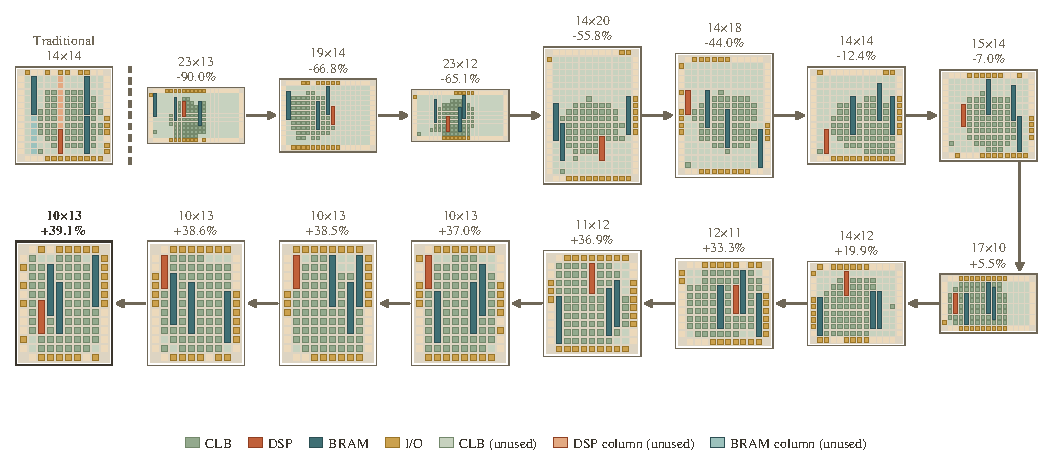
\includegraphics[width=0.98\textwidth]{fig_spree_timeline.pdf}
\caption{The training progression for \texttt{spree} (seed 123). Arrows
trace every episode that set a new best-so-far ADP reduction, left to right
across the top row and then right to left across the bottom row. Each panel
is a real VPR placement: saturated tiles are occupied, pale tiles are
provisioned but unused. Early episodes, still close to random exploration,
overshoot badly in both fabric size and ADP. Later episodes converge on a
compact, exactly-sized fabric (bottom left).}
\Description{Sixteen-panel grid showing the evolution of the spree fabric
layout: the traditional periodic architecture, separated by a dotted line
from fifteen RL-discovered layouts connected by arrows in chronological
order of when each set a new best ADP reduction, snaking left to right then
right to left, ending at the best layout found, with grid size and percent
ADP reduction labeled on each panel.}
\label{fig:layout}
\end{figure*}

\section{Conclusion}
\label{sec:conclusion}

We train a single graph-and-grid-conditioned RL policy that places H-blocks
and selects fabric aspect ratio, evaluated throughout against the real VTR
flow rather than a proxy. The same fixed checkpoint transfers zero-shot to
unseen benchmark circuits, including fabrics larger than anything in the
training pool, with a positive ADP reduction on every held-out circuit.

This is the practical case for a learned policy over per-instance search.
A GA restarts from scratch for every new circuit and incurs its full
VTR-evaluation cost each time, a cost that grows with circuit size; the
trained policy incurs that cost once, at training time, and reuses it
through a single rollout per new circuit. Its advantage therefore grows
with the number of circuits the same checkpoint is applied to, and is
largest on the large circuits where per-instance search is most expensive.

\bibliographystyle{ACM-Reference-Format}
\bibliography{references}

\end{document}
